\FloatBarrier
\section{Miary dla wierzchołków}
\begin{figure}[h]
	\centering
	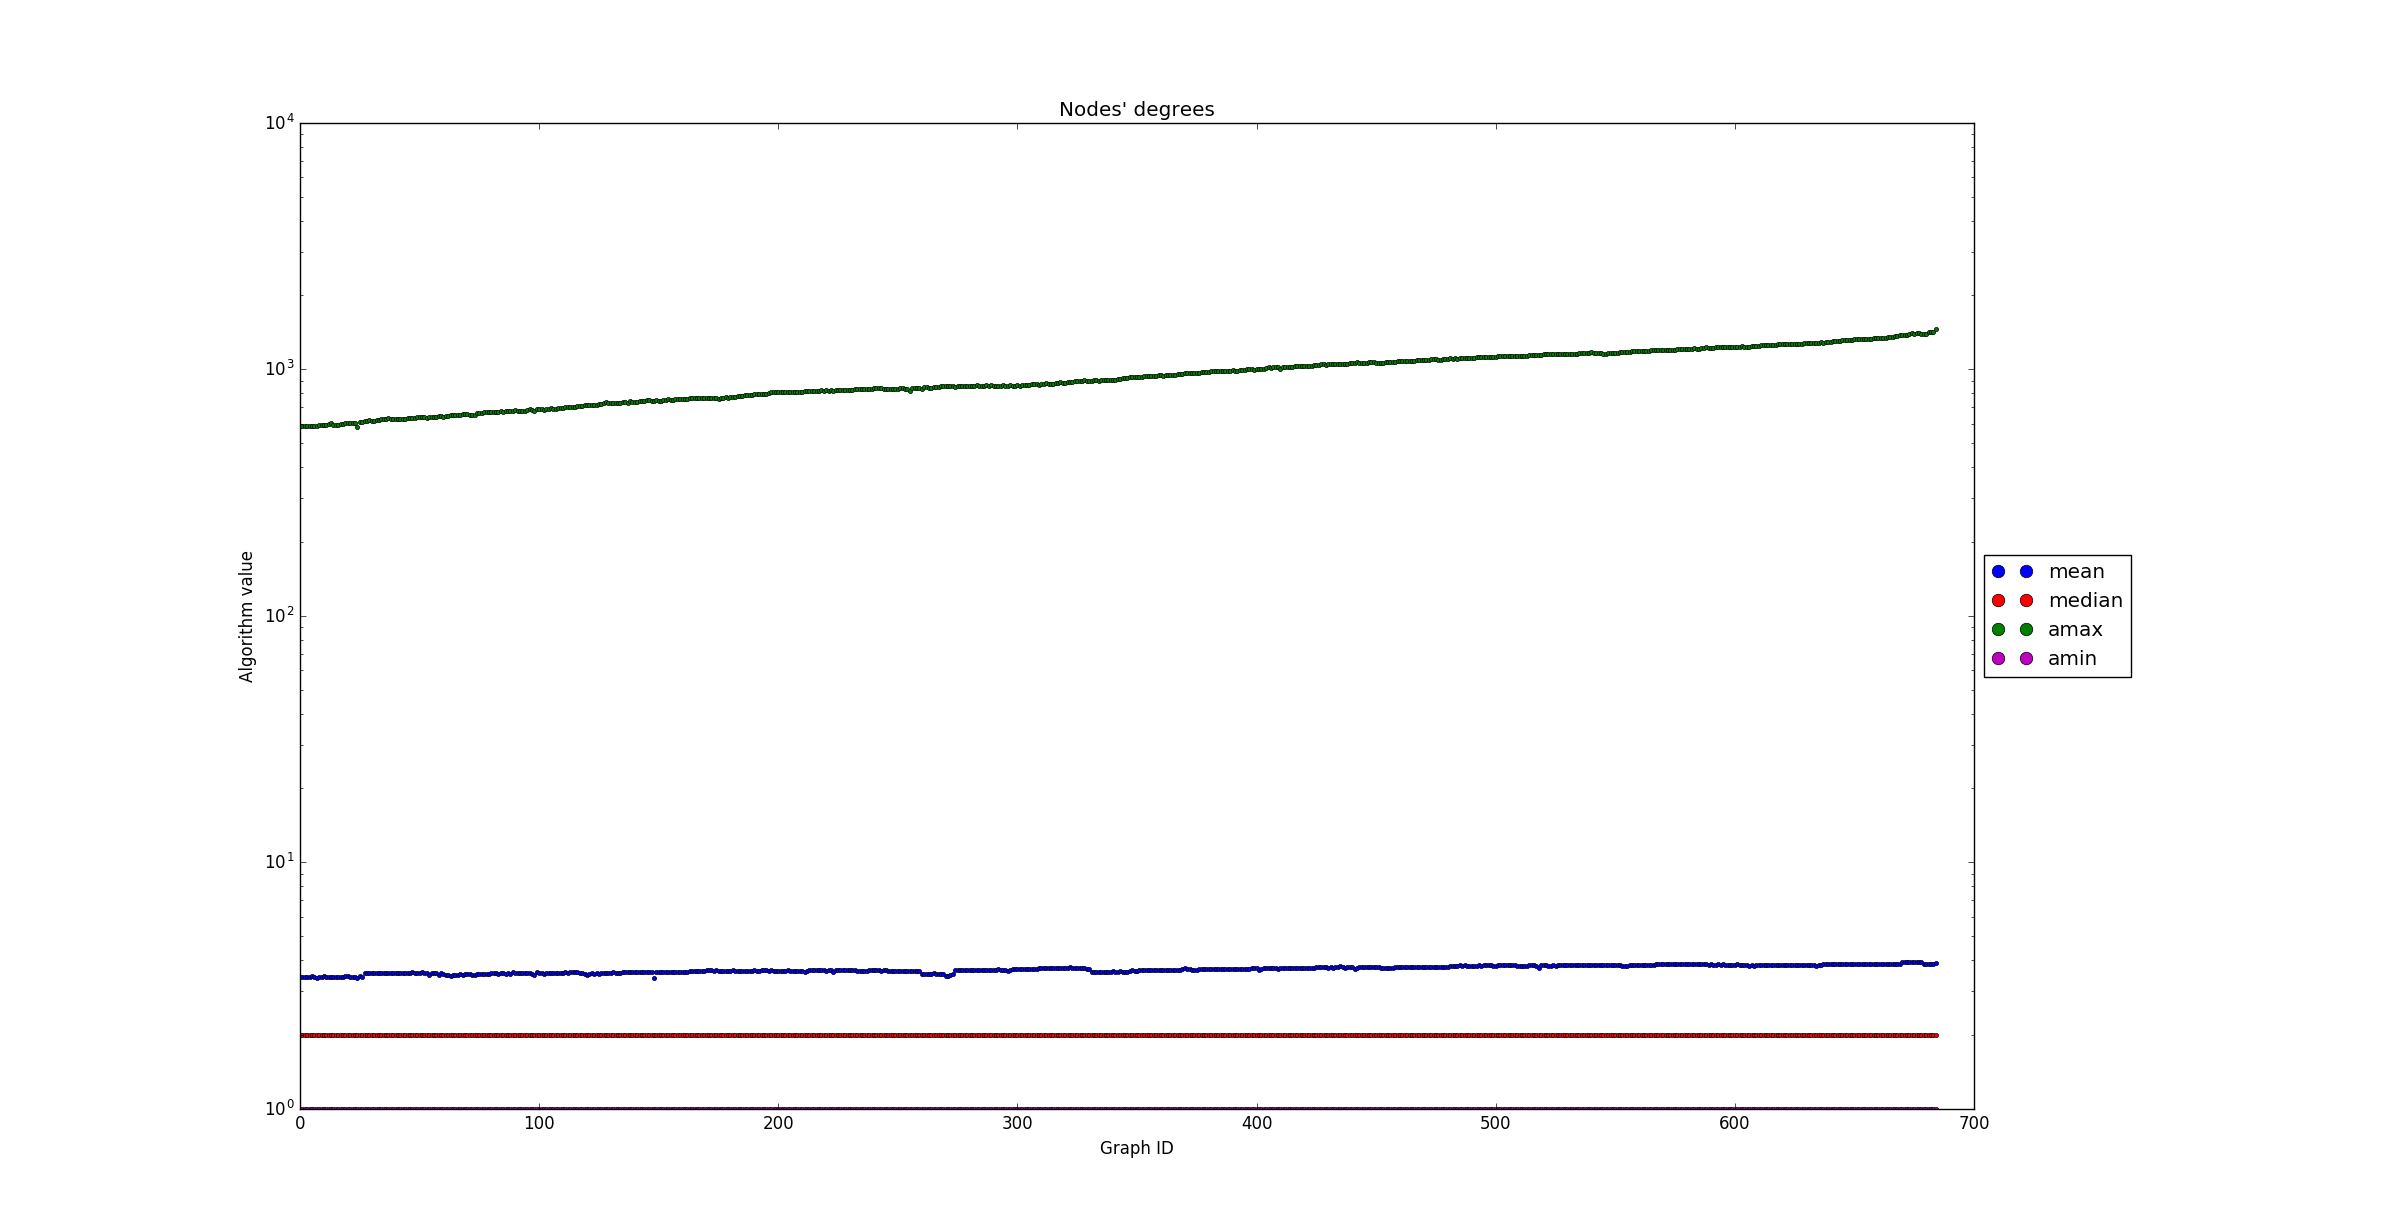
\includegraphics[width=\textwidth]{nodes_degrees}
	\caption{Stopnie wierzchołków}
\end{figure}
\FloatBarrier
\FloatBarrier
\begin{figure}[h]
	\centering
	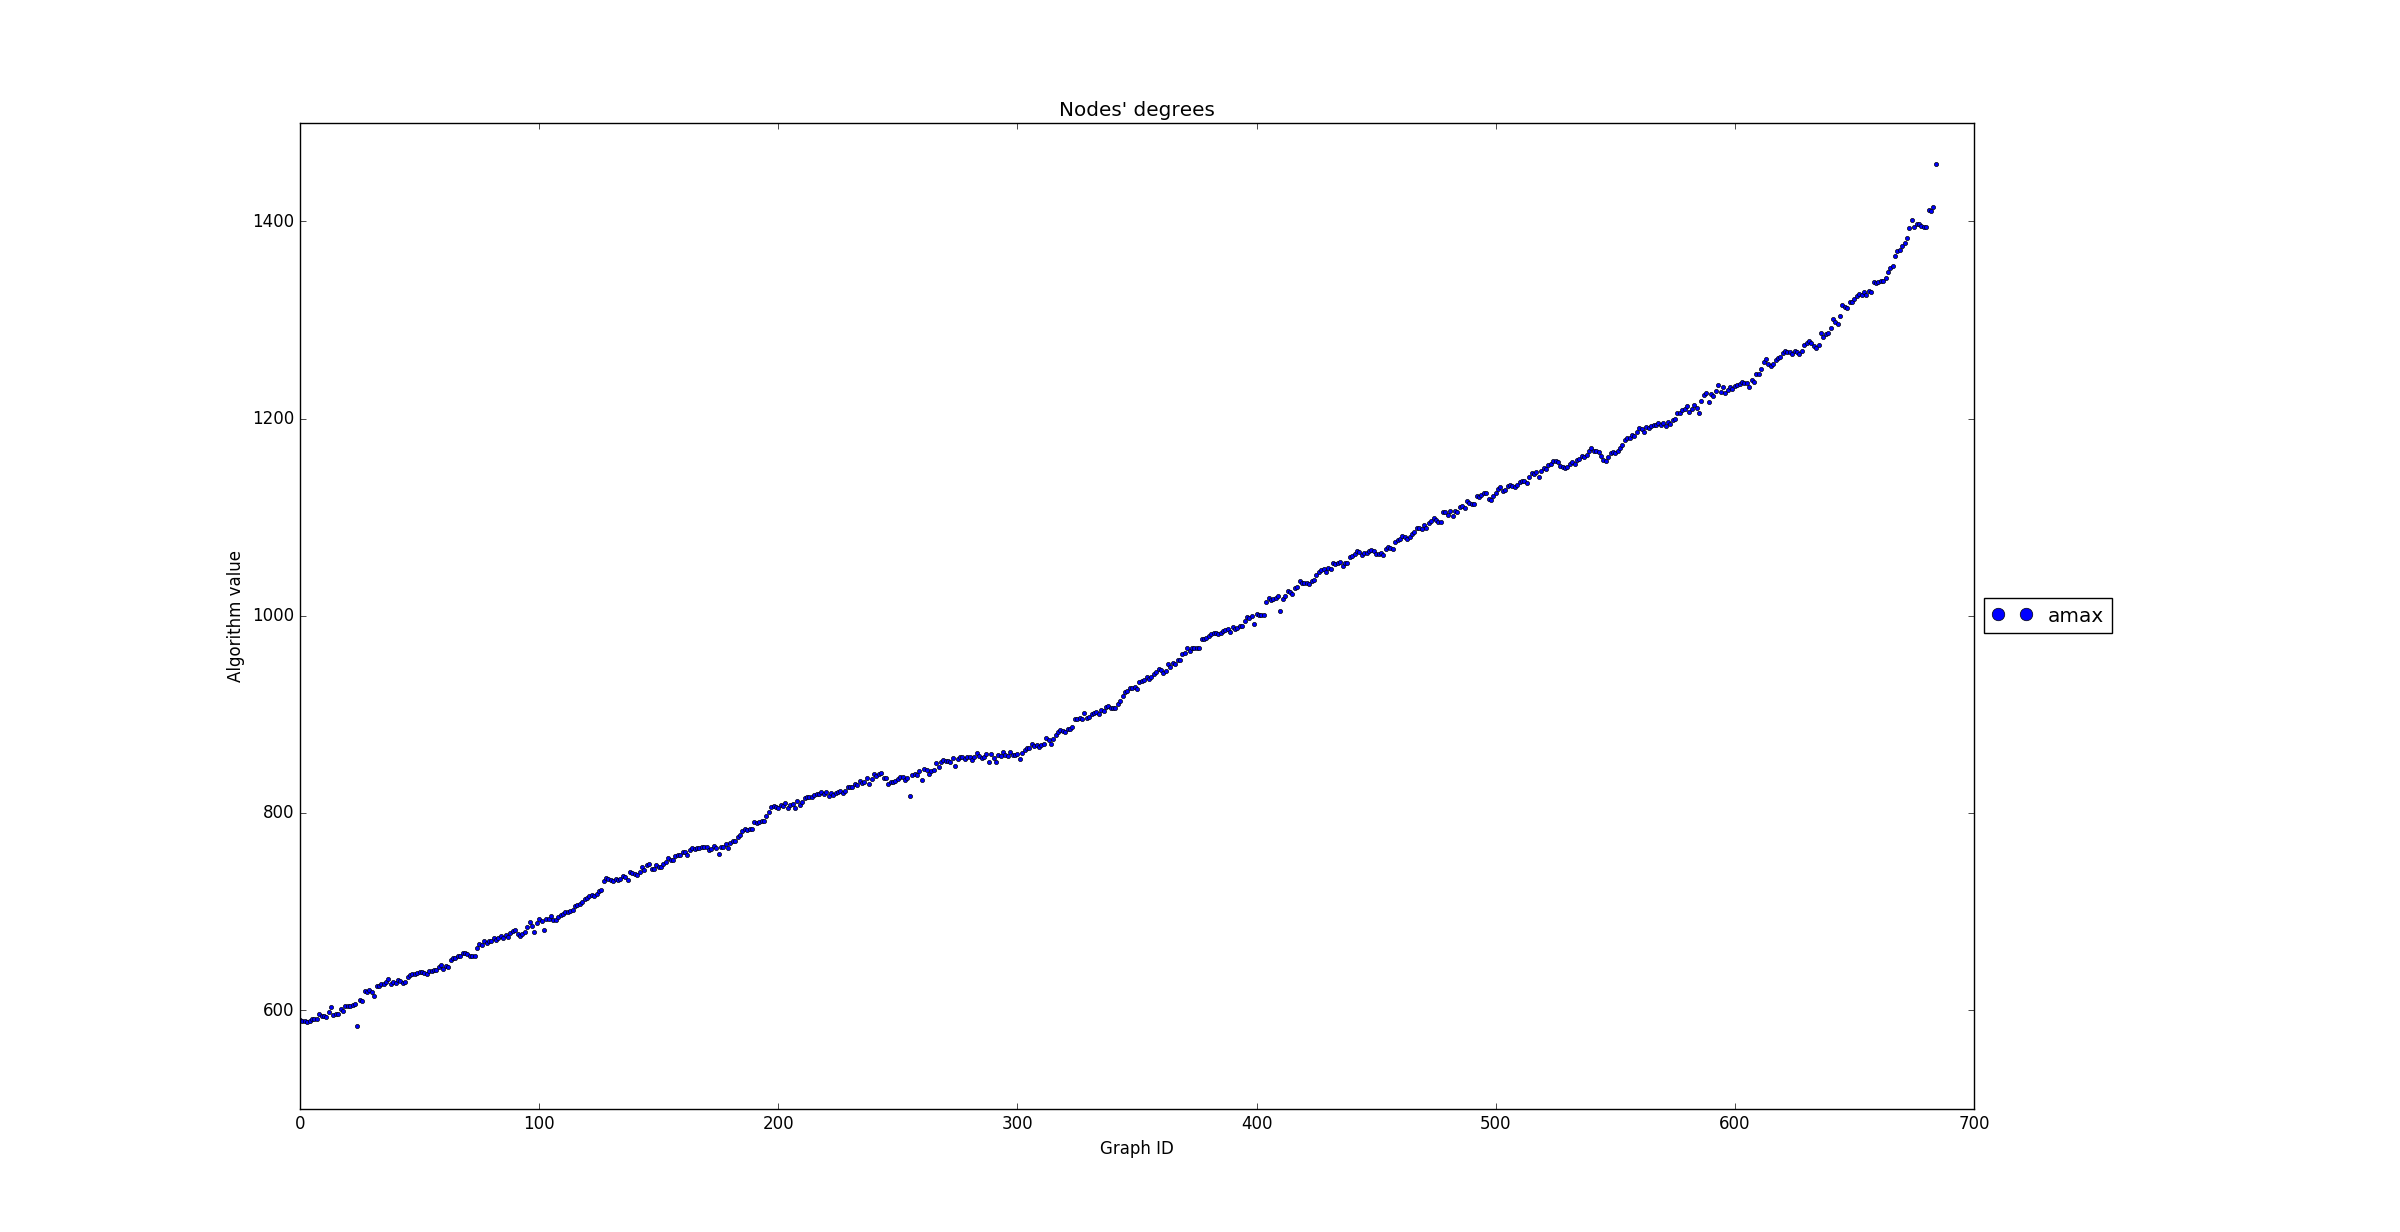
\includegraphics[width=\textwidth]{nodes_degree_max}
	\caption{Maksymalne stopnie wierzchołków }
\end{figure}
\FloatBarrier
\FloatBarrier
\begin{figure}[h]
	\centering
	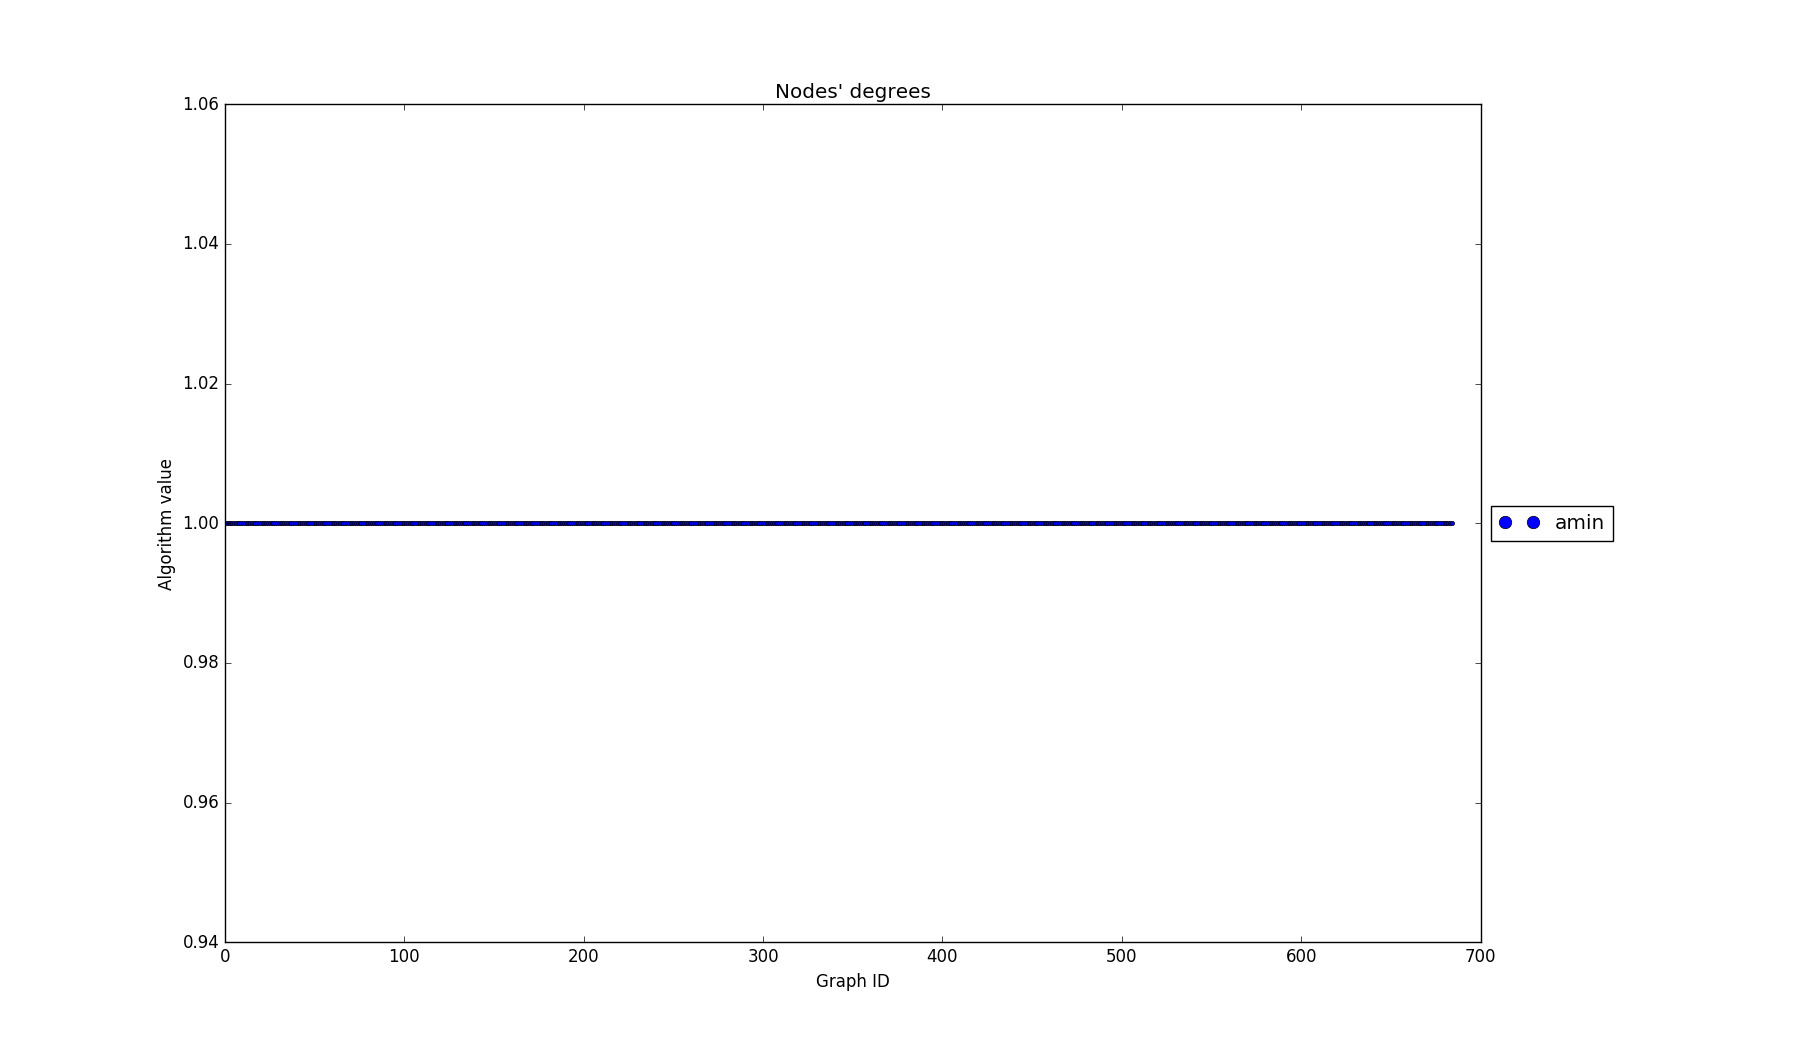
\includegraphics[width=\textwidth]{nodes_degree_min}
	\caption{Minimalne stopnie wierzchołków}
\end{figure}
\FloatBarrier\FloatBarrier
\begin{figure}[h]
	\centering
	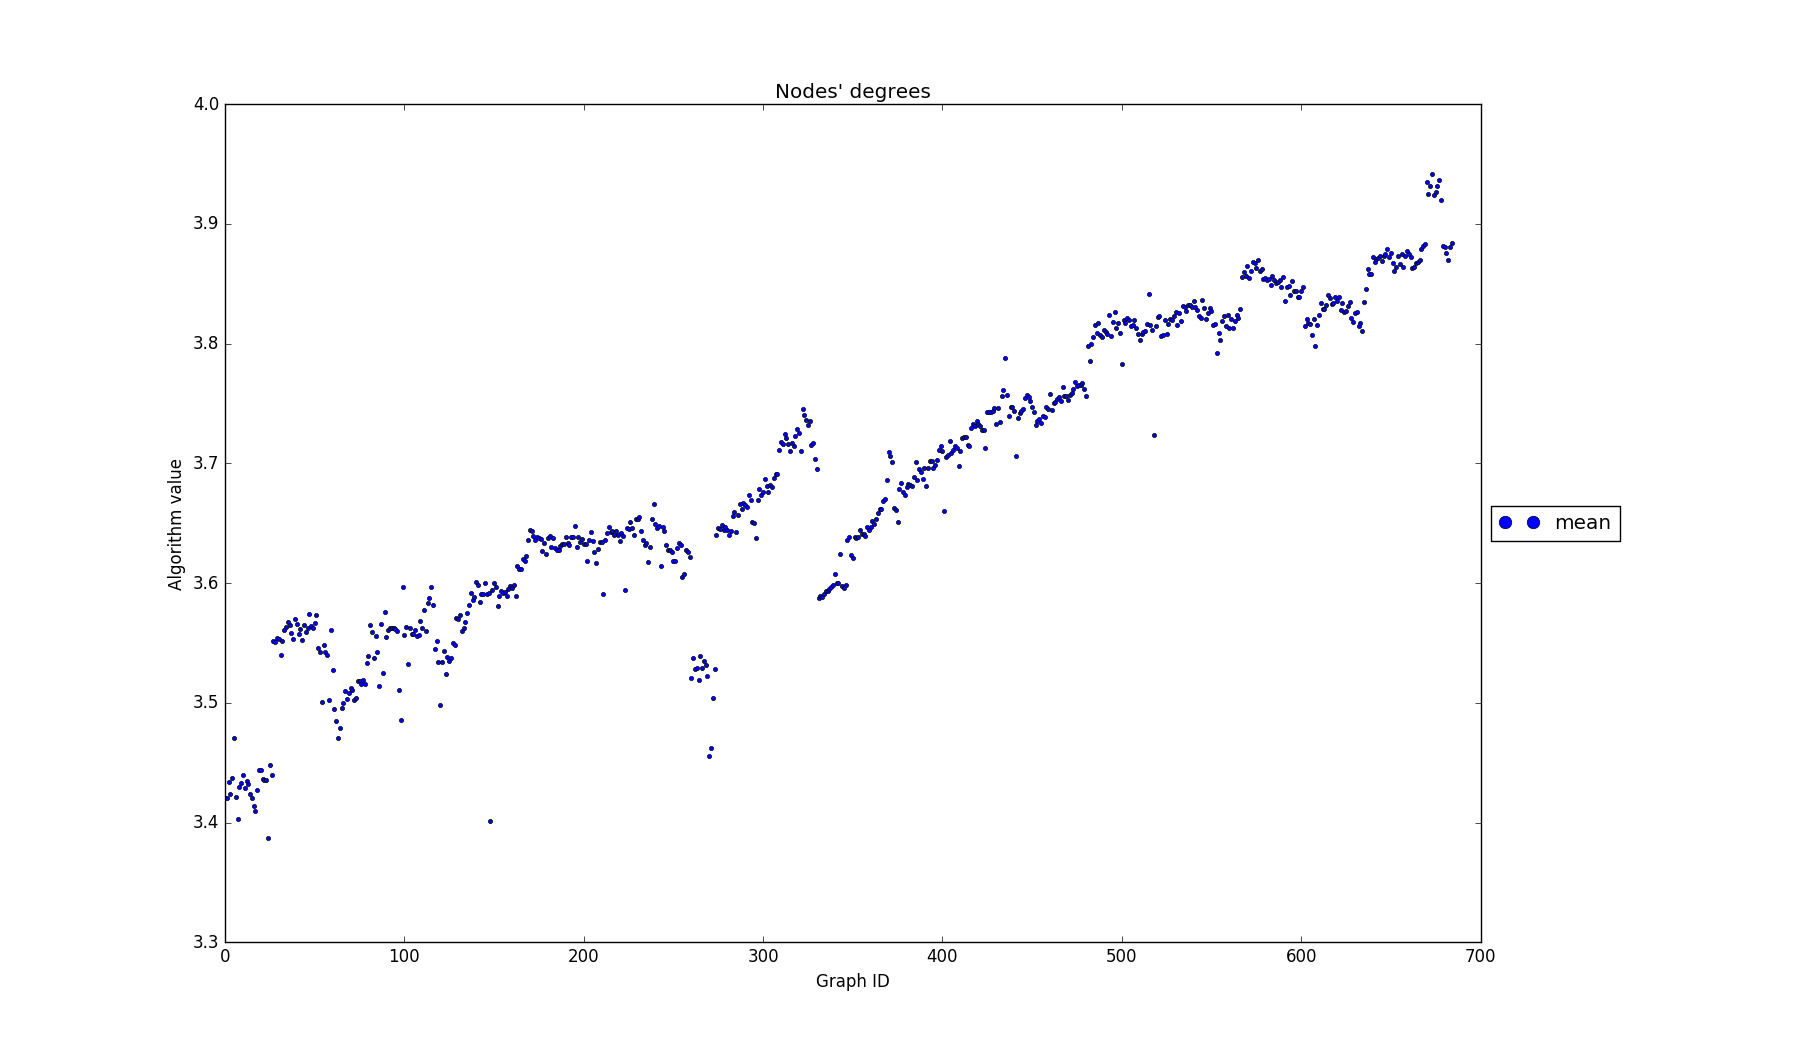
\includegraphics[width=\textwidth]{nodes_degrees_mean}
	\caption{Średni stopień wierzchołka w grafie}
\end{figure}
\FloatBarrier\FloatBarrier
\begin{figure}[h]
	\centering
	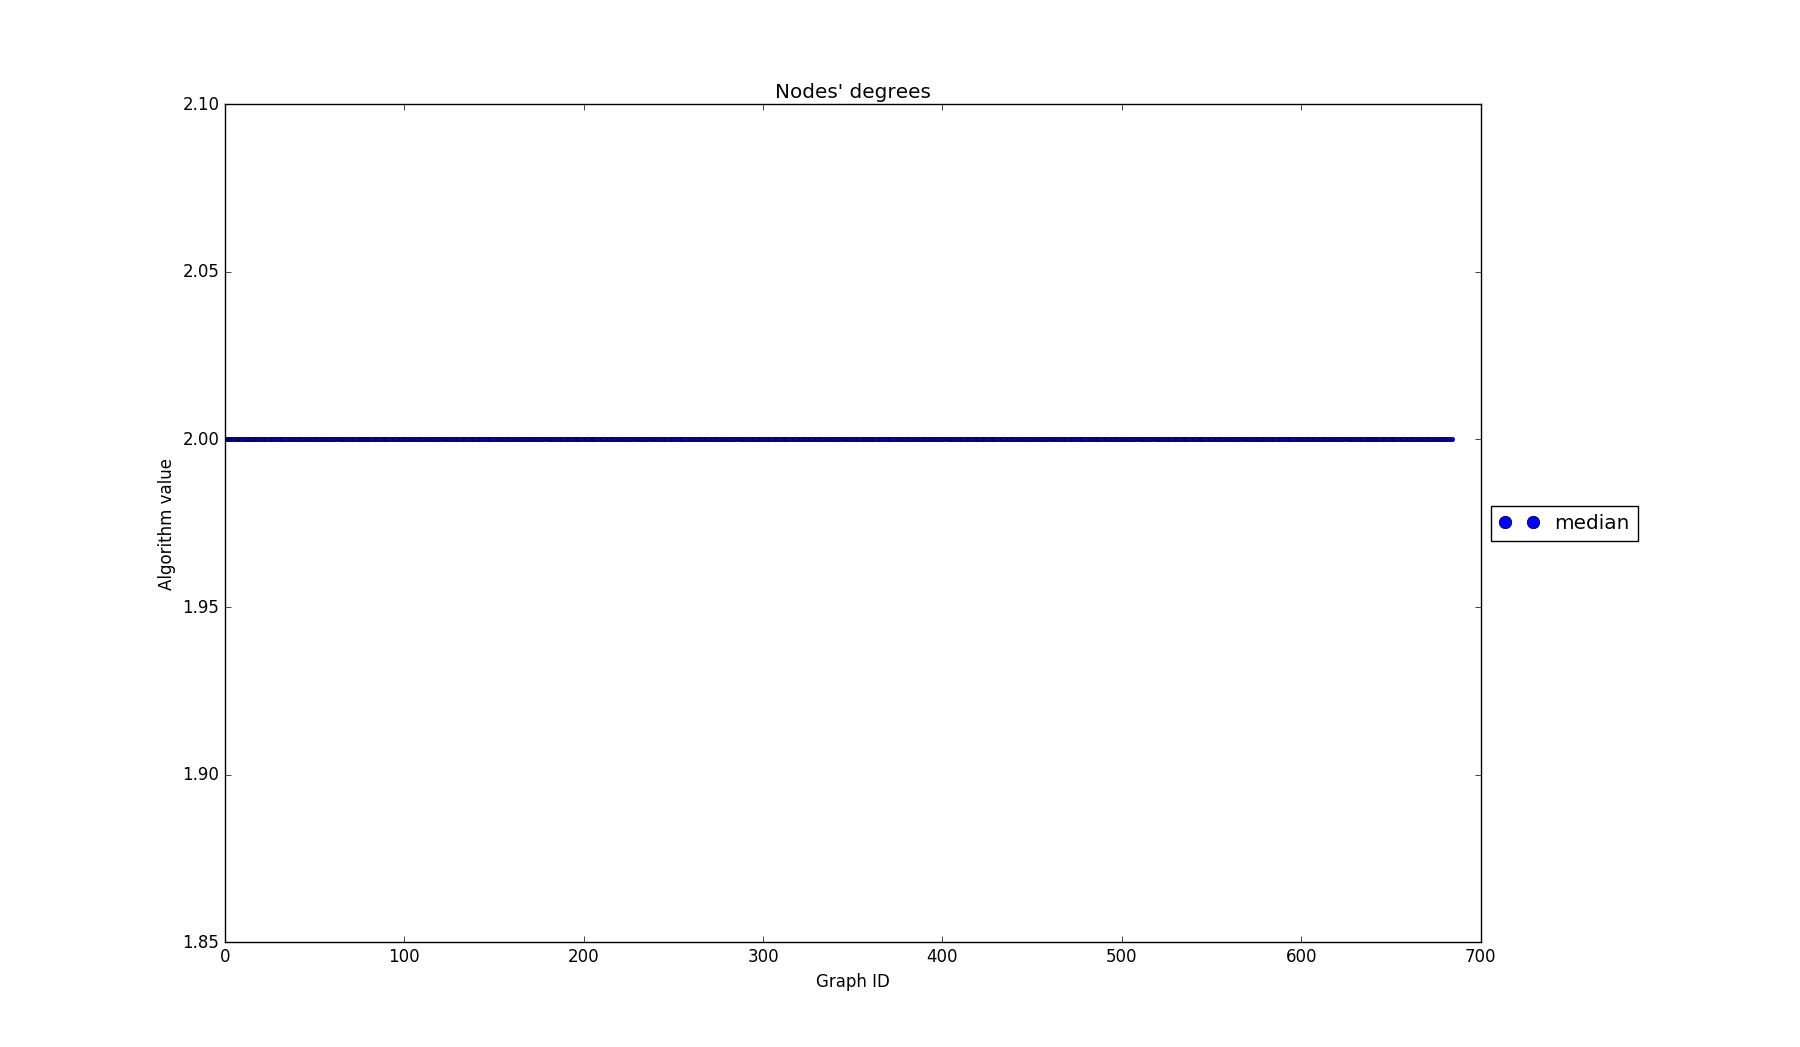
\includegraphics[width=\textwidth]{nodes_degrees_median}
	\caption{Mediana stopni wierzchołka}
\end{figure}
\FloatBarrier\FloatBarrier
\begin{figure}[h]
	\centering
	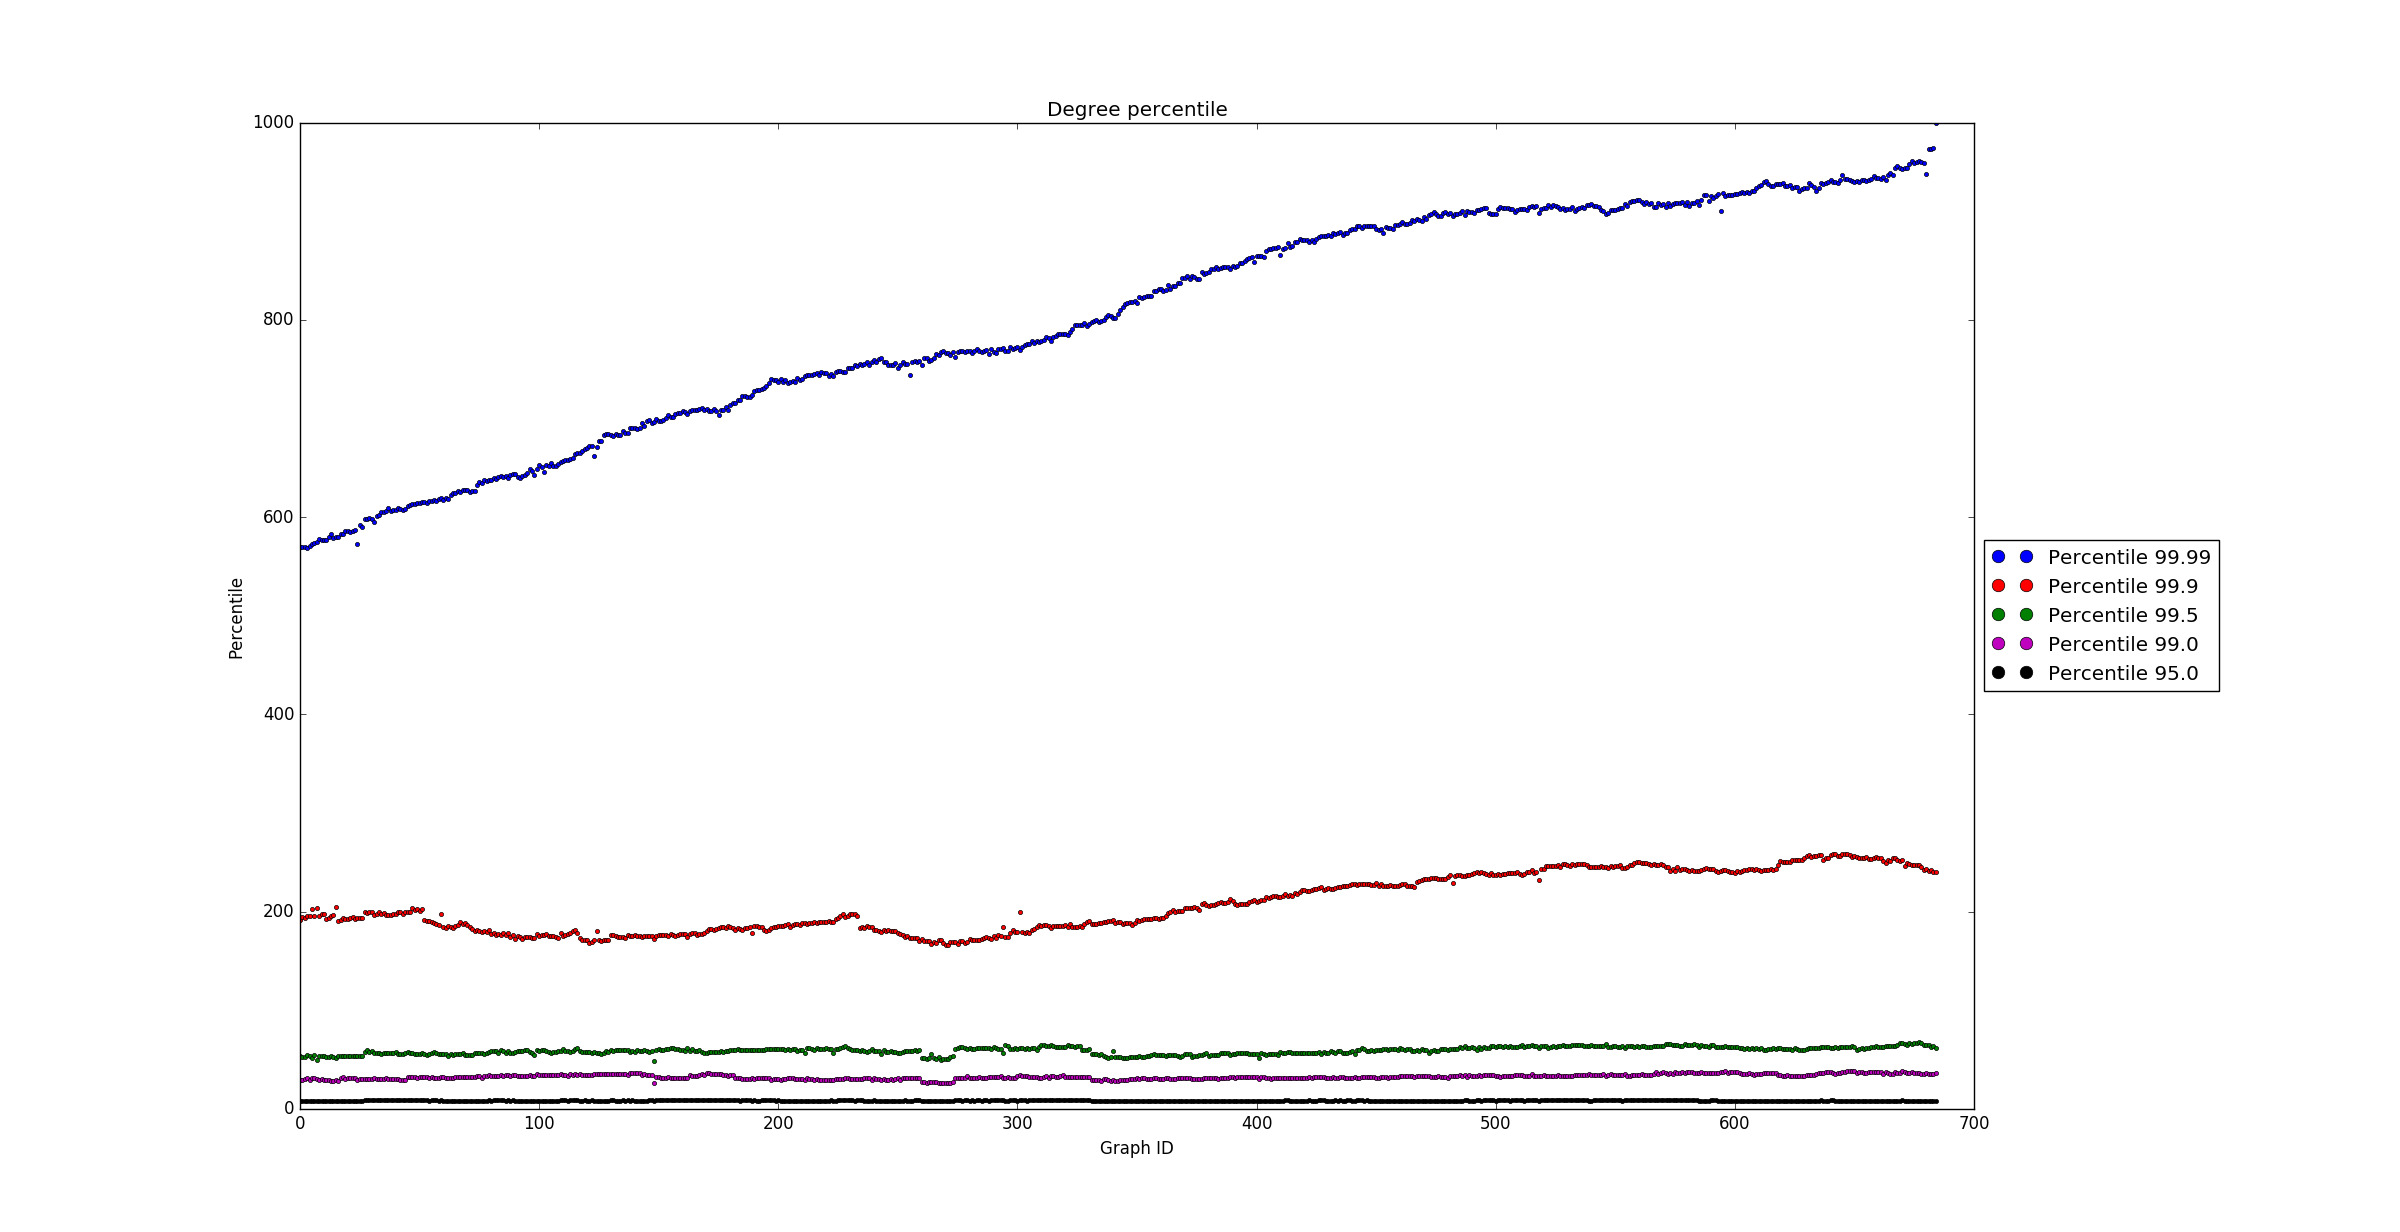
\includegraphics[width=\textwidth]{degree_percentiles}
	\caption{Percentyle dla stopni wierzchołka}
\end{figure}

Z powyższych wykresów wynika, że graf jest duży i ma relatywnie niską gęstość połączeń. Przez cały okres duża ilość wierzchołków (95\%) ma niski stopień, co przekłada się na niską średnią oraz medianę i może wpływać na wyniki algorytmów. 
\FloatBarrier\FloatBarrier
\newpage